% Created 2019-10-21 Пн 09:20
% Intended LaTeX compiler: pdflatex
\documentclass[11pt]{article}
\usepackage[utf8]{inputenc}
\usepackage[T1]{fontenc}
\usepackage{graphicx}
\usepackage{grffile}
\usepackage{longtable}
\usepackage{wrapfig}
\usepackage{rotating}
\usepackage[normalem]{ulem}
\usepackage{amsmath}
\usepackage{textcomp}
\usepackage{amssymb}
\usepackage{capt-of}
\usepackage{hyperref}
\usepackage[T2A]{fontenc}
\usepackage[a4paper,left=3cm,top=2cm,right=1.5cm,bottom=2cm,marginparsep=7pt,marginparwidth=.6in]{geometry}
\usepackage{cmap}
\usepackage{xcolor}
\usepackage{listings}
\usepackage{polyglossia}
\setdefaultlanguage{russian} \setotherlanguage{english}
\setmainfont{Liberation Serif}
\setsansfont{Liberation Sans}
\setmonofont[Contextuals=Alternate,Ligatures={TeX}]{Fira Code Regular}
\usepackage{spverbatim}
\author{Krutko Nikita / KrutNA}
\date{\today}
\title{}
\hypersetup{
 pdfauthor={Krutko Nikita / KrutNA},
 pdftitle={},
 pdfkeywords={},
 pdfsubject={},
 pdfcreator={Emacs 26.1 (Org mode 9.1.9)}, 
 pdflang={Russian}}
\begin{document}

\large
\thispagestyle{empty}
\begin{center}
\textbf{Национальный Исследовательский Университет ИТМО}\\
\textbf{Факультет Программной Инженерии и Компьютерной Техники}\\
\end{center}
\vspace{2em}
\begin{center}

\includegraphics[width=120pt]{itmo-logo.png}
\end{center}
\LARGE
\vspace{5em}
\begin{center}
\textbf{Вариант №82444}\\
\textbf{Лабораторная работа №2}\\
\Large
\textbf{по дисциплине}\\
\LARGE
\textbf{\emph{'Программирование'}}\\
\end{center}
\vspace{11em}
\large
\begin{flushright}
\textbf{Выполнил:}\\
\textbf{Студент группы P3113}\\
\textbf{\emph{Крутько Никита} : 242570}\\
\textbf{Преподаватель:}\\
\textbf{\emph{Письмак Алексей Евгеньевич}}\\
\end{flushright}
\vspace{4em}
\large
\begin{center}
\textbf{Санкт-Петербург 2019 г.}
\end{center}
\pagebreak{}
\setcounter{tocdepth}{3}
\tableofcontents
\vspace{2em}
\newfontfamily\lstcomment[Scale=0.6]{Fira Code Regular}
\newfontfamily\lstbasic[Scale=0.8,Contextuals=Alternate,Ligatures={TeX}]{Fira Code Regular}
\lstset{
  frame = shadowbox,
  commentstyle = \lstcomment\it\small,
  basicstyle = \lstbasic\small,
  numberstyle = \lstbasic\tiny,numbers=left,
  stringstyle = \lstbasic\it\small,
}
\section{Задание}
\label{sec:org1f20b90}
\subsection{Текст}
\label{sec:org0079e1f}
\small
Write your own pokemon classes based on Pokemon class for all given pokemons. Each pokemon kind should hae one or two types and standard base stats: HP, attack, defense, special attack, special defense and speed.

Pokemon classes should be inherited according to pokemon evolution chains.

Write your own Move classes based on PhysicalMove, SpecialMove and StatusMove classes for all give moves. Each move should have standard type, power and accuracy and implement standard move effects. Assign moves to pokemons according to given task. Pokemon level should be set to minimal one required to learn all given moves.

Use the simulation class Battle to create two pokemon teams (each pokemon should have a name) and start the battle.

Base classes, battle simulator and utility classes are packed in jar archive. Documentation in javadoc format is in the zip file.

All information about pokemon and move stats, evolution chains and so on you can find on \url{http://pokemondb.net}, \url{http://veekun.com/dex/pokemon}

\subsection{Комментарии}
\label{sec:orgccc63f0}
Task goal: Learn basic OOP principles using simple example and use them in your program.

TO DO:

Read documentation, pay special attention to Pokemon and Move classes. Later on working on lab continue to read documentation several times.
Download Pokemon.jar. You need to use it to compile and run your program. Don't unpack it. You should learn how to use third-party jar-files together with your program.
Write minimal working program and run it.
\lstset{language=Java,label= ,caption= ,captionpos=b,numbers=none}
\begin{lstlisting}
Battle b = new Battle();
Pokemon p1 = new Pokemon("Alien", 1);
Pokemon p2 = new Pokemon("Predator", 1);
b.addAlly(p1);
b.addFoe(p2);
b.go();
\end{lstlisting}
Create one of pokémon class according to your individual task. The class should inherit from base Pokemon class. You should set pokémon types and base stats in the constructor. Add your new pokémon to the team and start the battle.
Create one of move class

\subsection{Покемоны}
\label{sec:orgae59553}
\begin{center}
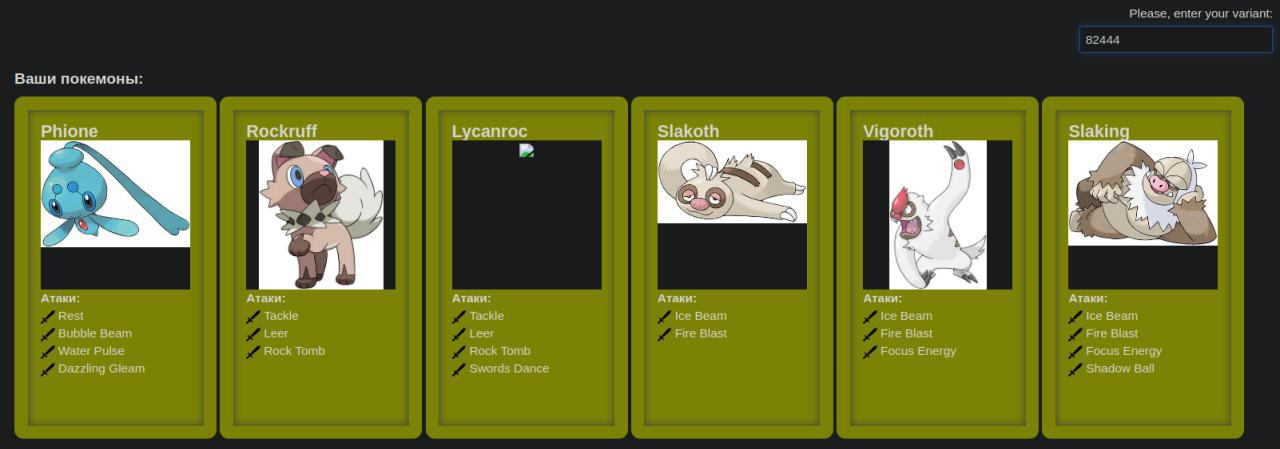
\includegraphics[width=.9\linewidth]{pokemons.jpg}
\end{center}

\section{Исходный код}
\label{sec:org38997be}
\subsection{Package: com.krutna.battler}
\label{sec:orgb7442f7}
\lstset{language=Java,label= ,caption={Battleground.java},captionpos=b,numbers=none}
\begin{lstlisting}
package com.krutna.battler;

import com.krutna.battler.pokemons.Lycanroc;
import com.krutna.battler.pokemons.Phione;
import com.krutna.battler.pokemons.Rockruff;
import com.krutna.battler.pokemons.Slaking;
import com.krutna.battler.pokemons.Slakoth;
import com.krutna.battler.pokemons.Vigoroth;
import ru.ifmo.se.pokemon.Battle;

public class Battleground {
  public static void main(String[] args) {
    Battle battle = new Battle();
    final String string = null;
    battle.addFoe(new Phione("'ошибаетесь, мухи на него слетаются по другой причине'", 99));
    battle.addAlly(new Rockruff("'джава'", 23));
    battle.addFoe(new Lycanroc("'deprecated с рождения'", 75));
    battle.addAlly(new Slakoth("'интерфейс не класс'", 38));
    battle.addFoe(new Vigoroth("'ты чёт его перегружаешь'", 38));
    battle.addAlly(new Slaking("'не стыдно, что от меня наследуешься?'", 38));
    battle.go();
  }
}
\end{lstlisting}

\subsection{Package: com.krutna.battler.moves}
\label{sec:orgcfd31db}
\subsubsection{Pacakge: com.krutna.battler.moves.physical}
\label{sec:org7fcecfb}
\lstset{language=Java,label= ,caption={RockTomb.java},captionpos=b,numbers=none}
\begin{lstlisting}
package com.krutna.battler.moves.physical;

import ru.ifmo.se.pokemon.Effect;
import ru.ifmo.se.pokemon.PhysicalMove;
import ru.ifmo.se.pokemon.Pokemon;
import ru.ifmo.se.pokemon.Stat;
import ru.ifmo.se.pokemon.Type;

public class RockTomb extends PhysicalMove {
  public RockTomb() {
    super(Type.ROCK, 60, 95);
  }

  @Override
  protected void applyOppEffects(Pokemon pokemon) {
    pokemon.addEffect(new Effect().stat(Stat.SPEED, 1));
  }
}
\end{lstlisting}
\lstset{language=Java,label= ,caption={Tackle.java},captionpos=b,numbers=none}
\begin{lstlisting}
package com.krutna.battler.moves.physical;

import ru.ifmo.se.pokemon.PhysicalMove;
import ru.ifmo.se.pokemon.Type;

public class Tackle extends PhysicalMove {
  public Tackle() {
    super(Type.NORMAL, 40, 100);
  }
}
\end{lstlisting}

\subsubsection{Package: com.krutna.battler.moves.special}
\label{sec:orgea242f2}
\lstset{language=Java,label= ,caption={BubbleBeam.java},captionpos=b,numbers=none}
\begin{lstlisting}
package com.krutna.battler.moves.special;

import ru.ifmo.se.pokemon.Effect;
import ru.ifmo.se.pokemon.Pokemon;
import ru.ifmo.se.pokemon.SpecialMove;
import ru.ifmo.se.pokemon.Type;

public class BubbleBeam extends SpecialMove {
  public BubbleBeam() {
    super(Type.WATER, 65, 100);
  }

  @Override
  protected void applyOppEffects(Pokemon pokemon) {
    pokemon.addEffect(new Effect().chance(0.1).turns(-1));
  }
}
\end{lstlisting}
\lstset{language=Java,label= ,caption={DazzlingGleam.java},captionpos=b,numbers=none}
\begin{lstlisting}
package com.krutna.battler.moves.special;

import ru.ifmo.se.pokemon.SpecialMove;
import ru.ifmo.se.pokemon.Type;

public class DazzlingGleam extends SpecialMove {
  public DazzlingGleam() {
    super(Type.FAIRY, 80, 100);
  }
}
\end{lstlisting}
\lstset{language=Java,label= ,caption={FireBlast.java},captionpos=b,numbers=none}
\begin{lstlisting}
package com.krutna.battler.moves.special;

import ru.ifmo.se.pokemon.Effect;
import ru.ifmo.se.pokemon.Pokemon;
import ru.ifmo.se.pokemon.SpecialMove;
import ru.ifmo.se.pokemon.Status;
import ru.ifmo.se.pokemon.Type;

public class FireBlast extends SpecialMove {
  public FireBlast() {
    super(Type.FIRE, 110, 85);
  }

  @Override
  protected void applyOppEffects(Pokemon pokemon) {
    pokemon.addEffect(new Effect().chance(0.1).condition(Status.BURN));
  }
}
\end{lstlisting}
\lstset{language=Java,label= ,caption={IceBeam.java},captionpos=b,numbers=none}
\begin{lstlisting}
package com.krutna.battler.moves.special;

import ru.ifmo.se.pokemon.Effect;
import ru.ifmo.se.pokemon.Pokemon;
import ru.ifmo.se.pokemon.SpecialMove;
import ru.ifmo.se.pokemon.Status;
import ru.ifmo.se.pokemon.Type;

public class IceBeam extends SpecialMove {
  public IceBeam() {
    super(Type.ICE, 90, 100);
  }

  @Override
  protected void applyOppEffects(Pokemon pokemon) {
    pokemon.addEffect(new Effect().chance(0.1).condition(Status.FREEZE));
  }
}
\end{lstlisting}
\lstset{language=Java,label= ,caption={ShadowBall.java},captionpos=b,numbers=none}
\begin{lstlisting}
package com.krutna.battler.moves.special;

import ru.ifmo.se.pokemon.Effect;
import ru.ifmo.se.pokemon.Pokemon;
import ru.ifmo.se.pokemon.SpecialMove;
import ru.ifmo.se.pokemon.Stat;
import ru.ifmo.se.pokemon.Type;

public class ShadowBall extends SpecialMove {
  public ShadowBall() {
    super(Type.GHOST, 80, 100);
  }

  @Override
  protected void applyOppEffects(Pokemon pokemon) {
    pokemon.addEffect(new Effect().chance(0.2).stat(Stat.SPECIAL_DEFENSE, 1));
  }
}
\end{lstlisting}
\lstset{language=Java,label= ,caption={WaterPulse.java},captionpos=b,numbers=none}
\begin{lstlisting}
package com.krutna.battler.moves.special;

import ru.ifmo.se.pokemon.Effect;
import ru.ifmo.se.pokemon.Pokemon;
import ru.ifmo.se.pokemon.SpecialMove;
import ru.ifmo.se.pokemon.Type;

public class WaterPulse extends SpecialMove {
  public WaterPulse() {
    super(Type.WATER, 60, 100);
  }

  @Override
  protected void applyOppEffects(Pokemon pokemon) {
    if (Math.random() < 0.2) {
      Effect.confuse(pokemon);
    }
  }
}
\end{lstlisting}

\subsubsection{Package com.krutna.battler.moves.status}
\label{sec:org59cfdf5}
\lstset{language=Java,label= ,caption={FocusEnergy.java},captionpos=b,numbers=none}
\begin{lstlisting}
package com.krutna.battler.moves.status;

import ru.ifmo.se.pokemon.Effect;
import ru.ifmo.se.pokemon.Pokemon;
import ru.ifmo.se.pokemon.Stat;
import ru.ifmo.se.pokemon.StatusMove;
import ru.ifmo.se.pokemon.Type;

public class FocusEnergy extends StatusMove {
  public FocusEnergy() {
    super();
    this.type = Type.NORMAL;
  }

  @Override
  protected void applySelfEffects(Pokemon pokemon) {
    pokemon.addEffect(new Effect().stat(Stat.ATTACK, -1));
  }
}
\end{lstlisting}
\lstset{language=Java,label= ,caption={Leer.java},captionpos=b,numbers=none}
\begin{lstlisting}
package com.krutna.battler.moves.status;

import ru.ifmo.se.pokemon.Effect;
import ru.ifmo.se.pokemon.Pokemon;
import ru.ifmo.se.pokemon.Stat;
import ru.ifmo.se.pokemon.StatusMove;
import ru.ifmo.se.pokemon.Type;

public class Leer extends StatusMove {
  public Leer() {
    super();
    this.type = Type.NORMAL;
    this.accuracy = 100;
  }

  @Override
  protected void applyOppEffects(Pokemon pokemon) {
    pokemon.addEffect(new Effect().stat(Stat.DEFENSE, 1));
  }
}
\end{lstlisting}
\lstset{language=Java,label= ,caption={Rest.java},captionpos=b,numbers=none}
\begin{lstlisting}
package com.krutna.battler.moves.status;

import ru.ifmo.se.pokemon.Effect;
import ru.ifmo.se.pokemon.Pokemon;
import ru.ifmo.se.pokemon.Stat;
import ru.ifmo.se.pokemon.Status;
import ru.ifmo.se.pokemon.StatusMove;
import ru.ifmo.se.pokemon.Type;

public class Rest extends StatusMove {
  public Rest() {
    super();
    this.type = Type.PSYCHIC;
  }

  @Override
  protected void applySelfEffects(Pokemon pokemon) {
    pokemon.addEffect(new Effect().turns(2).condition(Status.SLEEP));
    pokemon.addEffect(new Effect().stat(Stat.HP, -666));
  }
}
\end{lstlisting}
\lstset{language=Java,label= ,caption={SwordsDance.java},captionpos=b,numbers=none}
\begin{lstlisting}
package com.krutna.battler.moves.status;

import ru.ifmo.se.pokemon.Effect;
import ru.ifmo.se.pokemon.Pokemon;
import ru.ifmo.se.pokemon.Stat;
import ru.ifmo.se.pokemon.StatusMove;
import ru.ifmo.se.pokemon.Type;

public class SwordsDance extends StatusMove {
  public SwordsDance() {
    super();
    this.type = Type.NORMAL;
  }

  @Override
  protected void applySelfEffects(Pokemon pokemon) {
    pokemon.addEffect(new Effect().stat(Stat.ATTACK, -1));
  }
}
\end{lstlisting}

\subsection{Package: com.krutna.battler.pokemons}
\label{sec:org165f548}
\lstset{language=Java,label= ,caption={Lycanroc.java},captionpos=b,numbers=none}
\begin{lstlisting}
package com.krutna.battler.pokemons;

import com.krutna.battler.moves.status.SwordsDance;
import ru.ifmo.se.pokemon.Type;

public class Lycanroc extends Rockruff {
  public Lycanroc(String name, int level) {
    super(name, level);
    this.setType(Type.ROCK);
    this.setStats(75, 115, 65, 55, 65, 112);
    this.addMove(new SwordsDance());
  }
}
\end{lstlisting}
\lstset{language=Java,label= ,caption={Phione.java},captionpos=b,numbers=none}
\begin{lstlisting}
package com.krutna.battler.pokemons;

import com.krutna.battler.moves.special.BubbleBeam;
import com.krutna.battler.moves.special.DazzlingGleam;
import com.krutna.battler.moves.special.WaterPulse;
import com.krutna.battler.moves.status.Rest;
import ru.ifmo.se.pokemon.Pokemon;
import ru.ifmo.se.pokemon.Type;

public class Phione extends Pokemon {
  public Phione(String name, int level) {
    super(name, level);
    this.setStats(80, 80, 80, 80, 80, 80);
    this.setType(Type.WATER);
    this.setMove(new Rest(), new BubbleBeam(), new WaterPulse(), new DazzlingGleam());
  }
}
\end{lstlisting}
\lstset{language=Java,label= ,caption={Rockruff.java},captionpos=b,numbers=none}
\begin{lstlisting}
package com.krutna.battler.pokemons;

import com.krutna.battler.moves.physical.RockTomb;
import com.krutna.battler.moves.physical.Tackle;
import com.krutna.battler.moves.status.Leer;
import ru.ifmo.se.pokemon.Pokemon;
import ru.ifmo.se.pokemon.Type;

public class Rockruff extends Pokemon {
  public Rockruff(String name, int level) {
    super(name, level);
    this.setType(Type.ROCK);
    this.setStats(45, 65, 40, 30, 40, 60);
    this.setMove(new RockTomb(), new Tackle(), new Leer());
  }
}
\end{lstlisting}
\lstset{language=Java,label= ,caption={Slaking.java},captionpos=b,numbers=none}
\begin{lstlisting}
package com.krutna.battler.pokemons;

import com.krutna.battler.moves.special.ShadowBall;

public class Slaking extends Vigoroth {
  public Slaking(String name, int level) {
    super(name, level);
    this.setStats(150, 160, 100, 95, 65, 100);
    this.addMove(new ShadowBall());
  }
}
\end{lstlisting}
\lstset{language=Java,label= ,caption={Slakoth.java},captionpos=b,numbers=none}
\begin{lstlisting}
package com.krutna.battler.pokemons;

import com.krutna.battler.moves.special.FireBlast;
import com.krutna.battler.moves.special.IceBeam;
import ru.ifmo.se.pokemon.Pokemon;
import ru.ifmo.se.pokemon.Type;

public class Slakoth extends Pokemon {
  public Slakoth(String name, int level) {
    super(name, level);
    this.setType(Type.NORMAL);
    this.setStats(60, 60, 60, 35, 35, 35);
    this.setMove(new IceBeam(), new FireBlast());
  }
}
\end{lstlisting}
\lstset{language=Java,label= ,caption={Vigoroth.java},captionpos=b,numbers=none}
\begin{lstlisting}
package com.krutna.battler.pokemons;

import com.krutna.battler.moves.status.FocusEnergy;

public class Vigoroth extends Slakoth {
  public Vigoroth(String name, int level) {
    super(name, level);
    this.setStats(80, 80, 80, 55, 55, 90);
    this.addMove(new FocusEnergy());
  }
}
\end{lstlisting}

\section{Диаграмма классов реализованной объектной модели}
\label{sec:org2f84503}
\begin{center}
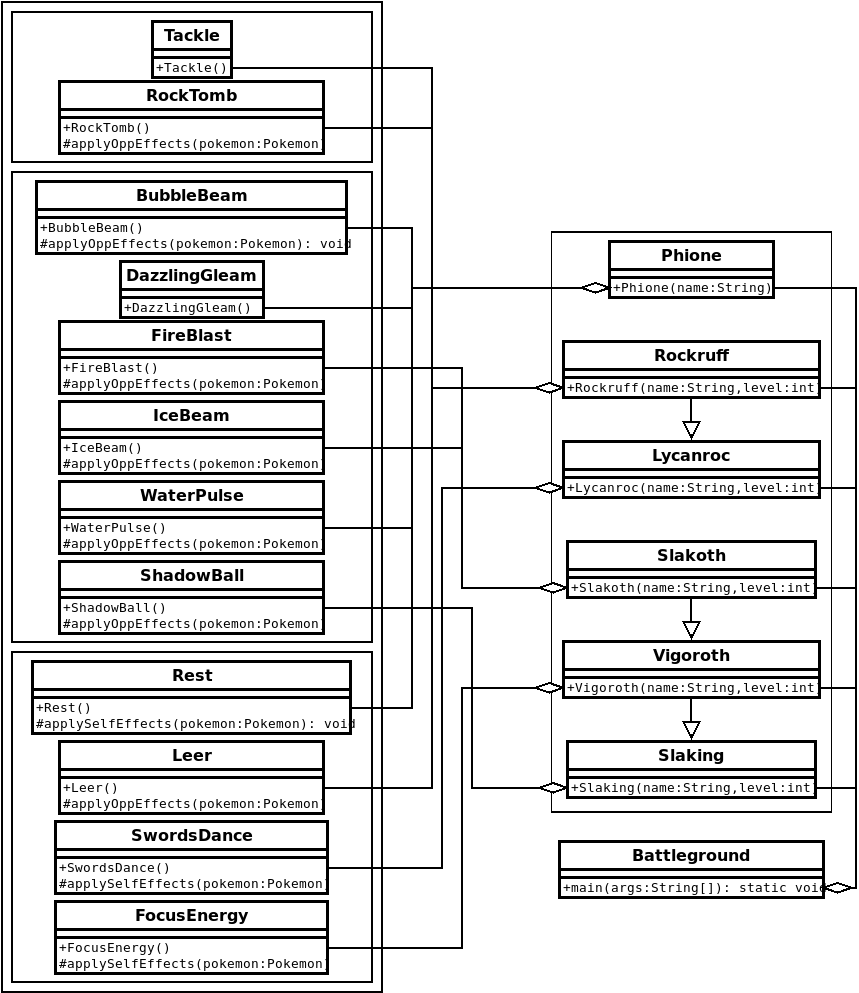
\includegraphics[width=.9\linewidth]{diagram.png}
\end{center}
\pagebreak{}

\section{Вывод программы}
\label{sec:orgbd3c5c6}
\scriptsize
\begin{tabular}{ll}
1 & Rockruff 'Джава' из команды зеленых вступает в бой!\\
2 & Phione 'Ошибаетесь, мухи на него слетаются по другой причине.' из команды фиолетовых вступает в бой!\\
3 & Phione 'Ошибаетесь, мухи на него слетаются по другой причине.' атакует.\\
4 & Rockruff 'Джава' теряет 285 здоровья.\\
5 & Rockruff 'Джава' теряет сознание.\\
6 & Slakoth 'интерфейс не класс' из команды зеленых вступает в бой!\\
7 & Phione 'Ошибаетесь, мухи на него слетаются по другой причине.' атакует.\\
8 & Slakoth 'интерфейс не класс' теряет 185 здоровья.\\
9 & Slakoth 'интерфейс не класс' теряет сознание.\\
10 & Slaking 'не стыдно, что от меня наследуешься?' из команды зеленых вступает в бой!\\
11 & Phione 'Ошибаетесь, мухи на него слетаются по другой причине.' атакует.\\
12 & Slaking 'не стыдно, что от меня наследуешься?' теряет 107 здоровья.\\
14 & Slaking 'не стыдно, что от меня наследуешься?' атакует.\\
15 & Phione 'Ошибаетесь, мухи на него слетаются по другой причине.' теряет 5 здоровья.\\
17 & Phione 'Ошибаетесь, мухи на него слетаются по другой причине.' атакует.\\
18 & Phione 'Ошибаетесь, мухи на него слетаются по другой причине.' засыпает\\
20 & Slaking 'не стыдно, что от меня наследуешься?' атакует.\\
21 & Phione 'Ошибаетесь, мухи на него слетаются по другой причине.' теряет 7 здоровья.\\
23 & Phione 'Ошибаетесь, мухи на него слетаются по другой причине.' восстанавливает 666 здоровья.\\
24 & Phione 'Ошибаетесь, мухи на него слетаются по другой причине.' атакует.\\
25 & Slaking 'не стыдно, что от меня наследуешься?' теряет 143 здоровья.\\
26 & Slaking 'не стыдно, что от меня наследуешься?' теряет сознание.\\
27 & В команде зеленых не осталось покемонов.\\
28 & Команда фиолетовых побеждает в этом бою!\\
\end{tabular}
\normalsize

\section{Вывод}
\label{sec:org6c014d7}
Я изучил основы ООП в Java. Поработал с \sout{ужасным} API библиотеки Pokemon.jar и выполнил на его основе задание 2ой лабораторной работы. Также изучил и использовал систему систему автоматической сборки Gradle и поставил её на helios.
\end{document}